\section{Introducción}

\begin{frame}\frametitle{Motivación}
  ¿Por qué vehículos sin conductor?
  \begin{itemize}
  \item La mayor cantidad de accidentes tienen como causa un error humano
  \item Se podría disminuir este número con vehículos sin conductor
  \item Menores tiempos de traslado mediante planeación de rutas óptimas y conducción sin distracciones
  \item Movilidad urbana más accesible
  \item Disminución de emisiones debido a una conducción óptima
  \end{itemize}
\end{frame}

\begin{frame}\frametitle{¿Cuándo un vehículos se considera autónomo?}
  La SAE propone seis niveles de autonomía:
  \[\]
  \textbf{Nivel 0 (\textit{No driving automation}):} El conductor es responsable de todas las tareas de conducción.
  \[\]
  \textbf{Nivel 1 (\textit{Driving assistance}):} El sistema de conducción automatizada toma control en situaciones muy específicas. Ejemplo: mantener cierta velocidad en carretera o frenar en automático ante un obstáculo.
  \begin{figure}
    \centering
    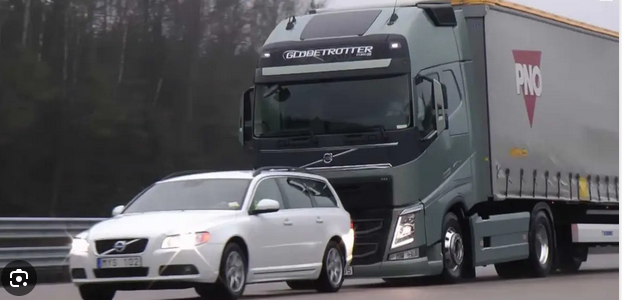
\includegraphics[width=0.5\textwidth]{Figuras/EjemploSAE1.png}
  \end{figure}
\end{frame}

\begin{frame}\frametitle{Niveles de autonomía SAE}
  \textbf{Nivel 2 (\textit{Partial driving automation}):} El auto puede realizar la mayor parte de tareas de conducción pero el conductor debe mantenerse atento durante toda la conducción. Ejemplo: Tesla.
  \begin{figure}
    \centering
    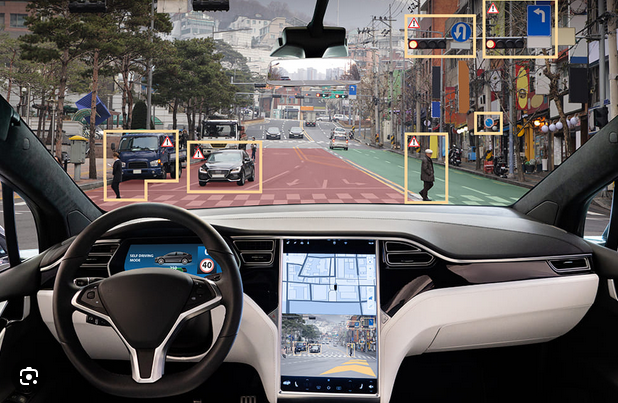
\includegraphics[width=0.5\textwidth]{Figuras/EjemploSAE2.png}
  \end{figure}
\end{frame}

\begin{frame}\frametitle{Niveles de autonomía SAE}
  \textbf{Nivel 3 (\textit{Conditional driving automation}):} El conductor puede desconectarse de la tarea de conducción bajo ciertos climas y carreteras. Todavía se requiere que el conductor resuelva ciertas situaciones de manejo. Ejemplo: Mercedes-Benz
  \begin{figure}
    \centering
    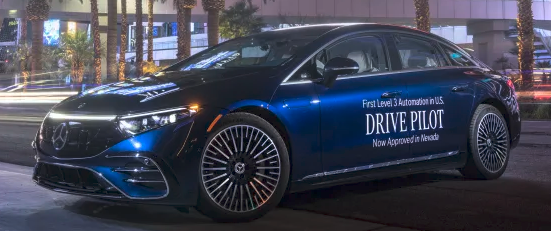
\includegraphics[width=0.7\textwidth]{Figuras/EjemploSAE3.png}
  \end{figure}
\end{frame}

\begin{frame}\frametitle{Niveles de autonomía SAE}
  \textbf{Nivel 4 (\textit{High driving automation}):} El vehículo es capaz de ejecutar funciones tácticas y operativas y es capaz de asegurarse automáticamente si los límites operativos se superan. El vehículo no es completamente autónomo pero el conductor no necesita responder ante fallas operativas. Ejemplo: \textbf{El TMR, pronto (esperemos)}
  \[\]
  \textbf{Nivel 5 (\textit{Full driving automation}):} No se requiere intervención humana y el sistema puede conducir sin restricciones de clima, carretera, horario o condición geográfica.  Ejemplo: \textbf{El TMR, pronto (esperemos)}
\end{frame}
